\clearpage
\section{Applications}
\label{sec:applications}

\subsection{Traffic Matrix Recovery}

As noted earlier it may be difficult to measure traffic matrices
directly, but we need to recover traffic matrices from measurements
before they can be used. The technique will obviously depend on the
available measurements, but there is a glut of works on the recovery
of traffic matrices, whether at the OD level, IE level or AS
level. Amongst these traffic matrices, IE traffic matrices are
relatively easier to recover, as measurements of these matrices are
available through SNMP link counts. Recovery of OD level traffic
matrices are fraught with challenges because at any point in time,
only a subset of IP traffic is seen by a network. There is no way to
know what goes on in the entire IPv4 address range, 
unless all measurements of the
global network were combined, but even so, the data from such an
endeavour would be massive and computationally intractable to
analyse, let alone accurate in the first place. Similarly, for AS level 
traffic matrices, the lack of measurements as well as error prone 
measurement tools lead to inaccurate recovery of these matrices.

The major challenge in recovering the IE traffic matrix from SNMP
measurements is that the problem is highly \emph{underconstrained}.
The set of linear equations \autoref{eq:observation} is
under-determined, \ie~there are many solutions to the
observations. Recall that the measurements themselves are subject to
error possibly due to poor data collection methods and poor vendor
implementation of SNMP polling.  They are also not fine-grained since
polling of the measurements is performed every 5 minutes (and the
polling intervals may not be perfectly synchronised across a whole
network). Clearly, any inference method is required to be robust
against these errors and uncertainties. 

The underconstrainedness of the problem may be mitigated by active
measures. One is direct measurement, using dedicated monitors or
in-built measurement software on routers such as NetFlow
\cite{NetFlow}.  Direct measurements at even a single point of ingress
results in measurement of an entire row of the traffic matrix,
drastically reducing the number of missing matrix entries. Another
interesting proposal is to change the IGP (Interior Gateway Protocol)
link weights over several snapshots within the measurement interval to
provide fresh sets of observations, thereby resulting in a system of
linear equations with a unique solution (full rank) out of the SNMP
measurements \cite{Nucci04IGPchange,soule07:_estim_dynam_traff_matric_using}. 
Both these techniques may be
impractical, either being too costly in the case of direct
measurements, or requiring direct intervention by the network operator
for IGP weight changes. Most proposals simply avoid these by settling
on a passive approach of inferring the traffic matrix straight from
SNMP data.

There are two main approaches to traffic matrix inference. The first is the deterministic approach, where
$\by$ is assumed to provide hard constraints, rather than statistical
data. Goldschmidt~\cite{Goldschmidt00LP} formulated this as
a Linear Program (LP) where the objective was designed 
 to find bounds on traffic matrix elements. In simple terms,
the LP finds the traffic matrix with the worst case upper and lower
bound on the traffic demand subject to constraints. Recall the vectorised 
traffic matrix $\bx$ has size $N(N-1)$. For the upper
bound, the LP model is defined with the objective function 
\be
\max_{\bx} \sum_{j=1}^{N(N-1)} \omega_j x_j,
  \label{eq:lp}
\ee

\noindent where $\omega_j$ is a weight for an OD pair $j$, also called
the coefficient of demand. There are three constraints to satisfy,
namely,
\begin{enumerate}
\item \textbf{observation constraints}:
\be
\sum_{j=1}^{N(N-1)} A_{ij} x_j \le y_i, \ i=1,2,\cdots, L,
\label{eq:observation_constraint}
\ee
\item \textbf{flow conservation constraints}:
\be
\sum_{\underset{\ell_1\ne\ell_2}{\ell_1 = i, \ell_2 =j,}} y_{\ell_1} A_{\ell_2 k} 
- \sum_{\underset{\ell_1\ne\ell_2}{\ell_1 = j, \ell_2 = i,}} y_{\ell_1} A_{\ell_2 k} = 
\begin{cases}
x_k, & \text{if $j$ is the source of $k$},\\
-x_k, & \text{if $j$ is the destination of $k$},\\
0, & \text{otherwise}.
\end{cases}
\label{eq:flow_conservation}
\ee
\item \textbf{non-negativity constraints}: $x_j \ge 0$, $j=1,2,\cdots, N(N-1)$.
\end{enumerate} 
\medskip 

\noindent Similarly, the lower bound is found by substituting the
maximisation operation in \eqref{eq:lp} with a minimisation operation.
The LP only produces a nontrivial solution if the lower bound and
upper bound on the traffic demand is greater than zero and less than
the observed total link count, \ie~$\sum_j y_j$.

Unfortunately, the utility of the LP is only restricted to small toy
problems. First, two linear programs have to be solved each time to
obtain the upper and lower bounds on traffic demands, which is
computationally expensive for large $N$.  Second, the LP was shown to have
terrible performance when tested on several types of traffic matrices
\cite{Medina02TMdirections}. Estimates of some traffic matrix entries
were in excess of 200$\%$, with most in excess of 100$\%$ error,
proving that while the LP may be useful for certain small topologies, in
general it is not considered a practical estimation method. The reason
for this is because the LP sets many estimated values to zero, resulting
in overcompensation for the rest of the estimated values in order to
meet the total traffic constraints. Third, there is a high sensitivity
of the solution to weight choices, which implies that different
solutions will be obtained depending on the chosen weights.

Instead, a more successful alternative is the use of statistical
models and regularisation, \ie\ treating the traffic matrix as a
realisation of a random process generated from a model. Regularisation
refers to the inference technique of imposing additional structural
assumptions on the problem to reduce
underconstrainedness. Regularisation methods are defined by four
components:
\begin{enumerate}
\item a \textbf{prior solution}, generated from a \emph{model}, 
\item a \textbf{model deviation} measure, used to compute the deviation of a feasible solution from the model, 
\item a \textbf{distortion} measure, used to compare the deviation of the model with the observations, and
\item an \textbf{adjustment step}, to ensure the constraints on the total traffic entering and exiting all ingress and egress nodes 
respectively, as well as non-negativity constraints, are satisfied.
\end{enumerate}
In terms of an optimisation procedure, solving the tomography problem is equivalent to
\begin{eqnarray}
\label{eq:opt_TMinverse}
\bx^\star = \argmin_{\bx \in \Real^{N(N-1)}} & R(\bx,\by) + \lambda d(\bx,\cM),
\end{eqnarray}
where $R(\cdot,\cdot)$ denotes the distortion measure,
$d(\cdot,\cdot)$ denotes the model deviation measure and $\lambda \ge
0$ is the penalty constant that amplifies the penalisation of a
feasible solution which strays too far away from the model\footnote
{Technically, $\bx$ comprises non-negative integers, but a relaxation
  to real numbers is used as it is easier to compute, especially when
  considering large traffic matrices.}. Typically, $R(\bx,\by) = \|\by
- \bA \bx\|_2$. Regularisation techniques are \emph{biased} to a
particular prior model. Thus, if the model is inconsistent, then the
estimator \eqref{eq:opt_TMinverse} would be inconsistent as
well. However, if the prior model chosen describes the final solution
somewhat accurately, then it is expected that the final estimate would
be fairly accurate.

As an example, suppose the prior
model, $\bx^{(0)}$, used is the gravity model, which can be derived
from link measurements by calculating the ingress and egress traffic
volumes (by summing link measures on the edge-links of the network). 
One proposed penalty~\cite{Zhang05InfoTh} is defined as 
\be d(\hat{\bx},\bx^{(0)}) = H(\hat{\bx}) + H(\bx^{(0)}) - H(\hat{\bx},\bx^{(0)}),
\label{eq:entropy_penalty}
\ee
where 
\be
H(\bx) = - \sum_{j=1}^{N(N-1)} \frac{x_j}{\sum_{k=1}^{N(N-1)} x_k} \log \frac{x_j}{\sum_{k=1}^{N(N-1)} x_k},
\label{eq:entropy}
\ee
is the empirical entropy, while 
\be
H(\bx,\bx^{(0)}) = \sum_{j=1}^{N(N-1)} \frac{x_j}{\sum_{k=1}^{N(N-1)} x_k} \log (\frac{x_j}{\sum_{k=1}^{N(N-1)} x_k} \Big/  
\frac{x^{(0)}_j}{\sum_{k=1}^{N(N-1)} x^{(0)}_k}),
\label{eq:joint_entropy}
\ee
is the joint empirical entropy, between the estimate and the prior model. The penalty function \eqref{eq:entropy_penalty} measures 
the uncertainty between the quantities $\bx$ and $\bx^{(0)}$, and is commonly known as the \emph{mutual information} 
\cite{Cover06InfoTheory}. The joint entropy term $H(\bx,\bx^{(0)})$ quantifies the uncertainty between $\bx$ and 
$\bx^{(0)}$. If $H(\bx,\bx^{(0)}) = 0$, then $\bx$ is statistically
independent of $\bx^{(0)}$. 

The approach is highly flexible: it can deal with the generalised
gravity model simply by using a new prior model and constraints
\eqref{eq:conditional_independence} are added to account for the
different traffic classes (access and peering traffic).

The penalty can be rewritten and thought of as the Kullback-Leibler
distance \cite{Cover06InfoTheory} between the estimate $\hat{\bx}$ and
the prior model $\bx^{(0)}$, implying that the estimation objective
seeks to preserve as much prior information from $\bx^{(0)}$ as
possible, while minimising $R(\bx,\by)$. This can be used directly, or
approximated, for instance as a weighted quadratic
\cite{Zhang03InfoSIGCOMM,Zhang03Fast}. 

Using suitable models, most of the existing inference methods can be
described in this framework (see \cite{Zhang05InfoTh} for details).
Or, other penalties can be used, such as the nuclear norm, given by
\be 
  d(\bX) =\|\bX\|_{\ast} = \sum_{i = 1}^r \sigma_i
  \label{eq:nuclear_penalty}
\ee
for low rank model recovery. 

The solution of the optimisation procedure is often adjusted after
regularisation using Iterative Proportional Fitting (IPF)
\cite{Deming40IPF}, so as to satisfy the observed total traffic
constraints and non-negativity constraints (those that were not
included in the regularisation for computational reasons). In
practice, the IPF is a very simple algorithm, performing fast even on
large traffic matrices. 

\begin{figure}[ht]
\Topology
\caption{Three example topologies where local traffic matrices provide
  benefits (motivated by the seminal figure in
  \cite{baran64:_distr}). \textbf{Left}: centralised, or star,
  topology, \textbf{Centre}: decentralised topology, \textbf{Right}:
  distributed topology.}
\label{fig:topology}
\end{figure}

% An important issue for regularisation methods is how much of an
% improvement regularisation would be over the initial ill-posed
% problem. Intuitively, if the model and constraints provide an
% information advantage, then it is easier to infer the traffic matrix.

Additional information can also be used, for instance, if some rows of
the matrix are known from measurements, then this eases the number of
variables to be estimated, making the problem a little simpler.
Another source of potential data is the collection of \textit{local
  traffic matrices} \cite{Varghese03Measure}, providing information on
traffic between interfaces of routers. We can see why this is useful
by considering the three network topologies in Figure
\ref{fig:topology}, with a centralised or star, a decentralised and a
distributed topology. If the network has a star topology, then the
entire traffic matrix is known if the local traffic matrix of the
router right in the centre is obtained. For the other two topologies,
collection of local traffic matrices in strategic places of the
topology is likely to reduce the underconstrainedness of the original
inference problem, though less (relative) information is provided the
more distributed the topology.  Local traffic matrices have been
demonstrated to provide a significant information boost in
\cite{Zhang03InfoSIGCOMM}, especially if the interfaces are
well-connected, and that is highly dependent on the underlying network
topology. If direct flow measurements from dedicated monitors are
available, they provide a huge boon as an entire row of an IE traffic
matrix would be revealed. In practice, however, these are generally
not available as they are deemed expensive. The advantage of the
regularisation method is that these additional information may be
incorporated easily via constraints.

Another issue is their computational tractability. Speed is an issue
for these algorithms, since traffic matrices are often large. Most
model deviation and distortion measures are chosen to be 
convex\footnote{Convex relaxations of a non-convex objective function is often
used as a substitute, for \eg, the nuclear norm is used in place of the rank function
to recover low rank matrices. Under these circumstances, it is crucial to 
note the assumptions of the model, so as to know when the recovered solution
is an excellent approximation of the true solution.}, with
linear constraints. In this way, problem \eqref{eq:opt_TMinverse} becomes a
convex optimisation problem, where many fast, scalable and efficient algorithms
have been developed to solve such problems \cite{Boyd04Opt}.

The discussions here only considered point-to-point traffic
matrices. For IE matrices, the point-to-multipoint matrix may be more
useful instead. Recall from the above that an ideal traffic matrix is
invariant to other network aspects to be useful for network
design. Unlike the point-to-point traffic matrix, the
point-to-multipoint matrix contains records on the amount of traffic
from one ingress point to a set of egress points. These sets are
chosen to preserve invariance under changes in the egress point, a
property much more useful for network planning. Inference of the
point-to-multipoint traffic matrices may be done in a similar fashion
to point-to-point IE matrices \cite{Zhang03InfoSIGCOMM}.

\subsection{Network Optimisation}

An ISP of a backbone network must ensure
each link in the network has adequate capacity. The consequences of
failure to provide  such capacity is congestion, and a resulting loss
of quality service, which in severe cases would result in loss of
customers. However, over-provisioning can be wasteful, and so
optimisation is used to strike the right balance between cost and
capacity.

Network optimisation and engineering 
\cite{Mitra05StochasticTE,Buriol03GAOSPF,Murphy02TE,Fortz02OSPF,Fortz03OSPF,Nucci07IGP,Uhlig04Implications,Feamster03BGPTE,Rexford06Route} involves several tasks with varying planning
horizons. Assuming node locations are fixed, in the long term, we plan
a network by considering the link locations, and capacity. We refer to
this as {\em network planning}. It may be categorised into two common
scenarios: \emph{incremental planning} on existing networks, or
\emph{green-fields planning} \cite{Roughan10Robust}. In the former,
the planning takes an evolutionary route, since the network designer
is constrained by the current existing network. Any upgrades to the
network are deliberately incremental, so as not to disrupt current
operations. Green-fields planning, as the name suggests, starts from
scratch: the entire network is designed from ground up. Shorter-term
network optimisation tasks include traffic
engineering~\cite{Roughan03TETM} and some potential routing schemes.

As an illustration of the use of a traffic matrix for testing routing schemes, 
consider a simple example of a topology with 
three nodes in \autoref{fig:demands}. The traffic matrix is given by
\ben
\bX = 
\left(
\begin{array}{ccc}
0 & 1 & 4\\
2 & 0 & 2\\
3 & 2 & 0
\end{array}
\right).
\een
The path distances from PoP 1 to 2, 1 to 3 and 2 to 3 is 1, 2 and 4 respectively. The goal is 
to find the shortest path routing based on the traffic matrix and the topology. Recall
that the link loads may be expressed as $\by = \bA \bx$, where 
$\bx = (1,4,1,2,3,2)^\T$ is the vectorised
form of $\bX$, without including self-traffic. The routing matrix $\bA$ 
here is size 3 by 6, since there are 3 links and 
6 flows, as we do not consider self-traffic. Each element is either 0 or 1 as the
flows are assumed to be delivered whole. The capacity of each link is assumed to be
infinite, or limitless.

Thus, finding the routes may be cast as the optimisation problem
(integer program) with a simple cost function based on path distance
\be
\begin{array}{ccc}
\bA^{\star} &= \displaystyle \argmin_{{A_{i,j} \in \{0,1\}, \forall i,j}} & y_{1,2} + 2y_{1,3} + 4y_{2,3}\\
& \text{ subject to} & \by = \bA \bx.
\end{array}
\label{eq:minKL}
\ee
The solution in this case is a simple one with 
\ben
\bA^\star = 
\left(
\begin{array}{cccccc}
1 & 0 & 1 & 1 & 0 & 1\\
0 & 1 & 0 & 1 & 1 & 1\\
0 & 0 & 0 & 0 & 0 & 0
\end{array} 
\right).
\een
The example presented is a simple, trivial one. In practice, networks have a larger
topology and additional costs may be included, such
as bandwidth utilisation of each link so as to minimise the maximum utilisation of the network,
QoS constraints, and constraints on the maximum capacity of each link. For instance, 
if the maximum capacity of the link from PoP 1 to 3 is at most 4 \ie~$y_{1,3} \le 4$, 
then the routing matrix above is no longer a 
feasible solution. The new solution must incorporate the link from PoP 2 to 3 to conform to 
constraints (assuming the link 2 to 3 has adequate capacity).

\begin{figure}
  \begin{center}
    \begin{center}
\tikzstyle{PoP} = [right,circle, draw]
\tikzstyle{line} = [draw]
\tikzstyle{dotline} = [draw,dotted]
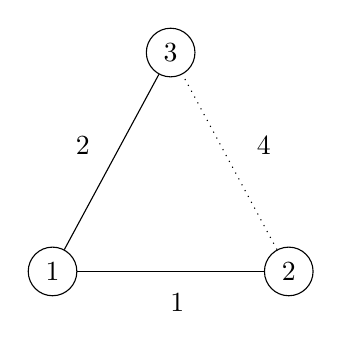
\begin{tikzpicture}
	\node (pop1) at (0.0,0.0) [PoP] {1};
	\node (pop2) at (3.0,0.0) [PoP] {2};
	\node (pop3) at (1.5,2.78) [PoP] {3};
	\path[line](pop1) -- (pop3);
	\path[line](pop1) -- (pop2);
	\path[dotline](pop2) -- (pop3);
	\node  at (0.7,1.6) {2};
	\node  at (1.9,-0.4) {1};
	\node  at (3.0,1.6) {4};
\end{tikzpicture}
\end{center}


    \caption{Example of a simple network of three PoPs and path distances of each link. The shortest path
    routes chosen are from PoP 1 to 2, and 
    from PoP 1 to 3, as these paths have the lowest distance (corresponding to the thick lines).
      \label{fig:demands}}    
  \end{center}
\end{figure}

In all of the above mentioned tasks, one of the key ingredients is the traffic
matrix. The reason these matrices are so useful comes down to {\em
  invariance}. The traffic on a particular link obviously varies as
the links in the network change. However, an ideal traffic matrix is
invariant to other aspects of the network such as the network topology
and underlying routing protocols. Invariance allows the design to be
varied without the inputs to the process changing.  To a certain
extent, the IE traffic matrix satisfies the invariance property, but
it is far from perfect for some tasks, most notably it is highly
sensitive to external routing changes and some internal changes
\cite{Teixeira05TMRoute,Teixeira04PotatoSIG}.  The OD matrix is in
some sense preferable \cite{Alderson06Topology}, but harder to measure
in most cases.  The point-to-multipoint IE matrix (discussed in the
previous section) is a useful compromise.

Furthermore, a network operator would require a prediction of the
traffic matrix out to the level of the planning horizon for a
task. Any forecast depends on the time scale involved and the
underlying model used. At short time scales, say minutes, stationarity
may be a reasonable approximation, and there are therefore many time
series approaches the problem. On time scales of hours to days to
weeks, the cyclostationary nature of the data must be included. The
temporal models presented earlier can provide such predictions.  For
instance, with the model \eqref{eq:temporal_model}, we can estimate
the average traffic at some time in the future by simply extrapolating
the mean. Longer-term prediction often focusses purely on the
large-scale trend $L(t)$ (see \autoref{ssec:temporal_modelling}), 
often captured using a simple growth model (linear 
or exponential) and regression. In all cases,
historical data is needed, usually several times as long as the
prediction interval.

In addition, whenever performing prediction we should provide an 
estimate of variances, or confidence intervals, though this component of the
problem has not been well-studied in the specific context of traffic
matrices. 


% Current routing algorithms require some knowledge of the traffic
% matrix to determine the paths of the traffic flows in the network.
% Typically, link state routing protocols such as Open Shortest Path
% First (OSPF) or Intermediate System-Intermediate System (IS-IS) are
% used for intra-domain routing, while the Border Gateway Protocol (BGP)
% is utilised for inter-domain routing. Regardless, these algorithms
% depend on the network topology and the traffic matrix. For example,
% with BGP, the operator needs to know the best egress point to route
% the traffic out of the network. By knowing both the set of ingress
% nodes and their traffic demands, as well as the topology, the best BGP
% configuration may be determined. Tests of new routing protocols on
% network topologies also require knowledge of the traffic
% matrix. Furthermore, these protocols can be tested on artificially
% synthesised traffic matrices based on a current model of the traffic.

% In day-to-day tasks, the network operator requires a picture of what
% is happening in the network. If a link becomes congested, then the
% traffic matrix at the link level helps a network operator identify the
% blockage and take necessary steps to correct the situation. In this
% situation, routing information also plays vital role, as weight
% changes are required to re-route a portion of the traffic to less
% congested links. Inference algorithms play an important role here, as
% inferred traffic matrices from SNMP measurements may be used for these
% tasks. An empirical study \cite{Roughan03TETM} proved that despite the
% inaccuracies of the recovered traffic matrices, these estimated
% traffic matrices still yield remarkably good solutions for traffic
% engineering tasks. Since mosts traffic engineering tasks revolve
% around large aggregate flows, as long as inaccuracies of the large
% flows are kept controlled and minimal, these estimated traffic
% matrices are good enough for network optimisation.


\subsection{Reliability Analysis}

Traffic matrices may also be used to conduct reliability analyses,
where the effect (on traffic) or network failures is considered. A
basic task in most network design is to create redundant paths to
carry traffic in case of failure, but if high reliability is required,
then an operator should also ensure that there is sufficient capacity
in the network to carry this traffic along its alternate paths.  For
more details of this task see \cite{Roughan10Robust}.

\subsection{Anomaly Detection}

In reality, not all traffic of a network is
legitimate. Various attacks may be launched: DDoS attacks \cite{Patrikakis04DDoS}
or worm outbreaks such as the Nimda worm \cite{Nimda}. Non-malicious, but equally
violent spikes in traffic may be caused by a flash crowd or
implementation bugs. We call these surges \textit{anomalies}, and if they catch
a network operator by surprise they can congest networks, causing
untold damage to daily network activities. Other types of anomalies
may cause drops in traffic, again resulting in performance problems.

All these anomalies may be rare, but the potential damage can be
tremendous. It is for these reasons network operators strife to detect
anomalies, with the hope of protecting their networks from these
harmful effects. 

Although network equipment vendors do provide some form of fast
detection and diagnosis mechanisms, these features are generally not
adequate for the problems listed above. Consequently, methods were
developed to counter anomalies. One approach is to use detailed
(packet level) traces and signature-based detection to detect known
attacks, but this does not help if the attack is unknown (in advance)
or if the necessary measurements are not available. Other techniques
infer statistical anomalies from the traffic flow data or SNMP
measurements. Traffic matrices play an important role in this respect,
since these matrices record traffic volumes across a whole network.

The basic principle of anomaly detection is to define a \emph{baseline
  operating condition} of the network, by establishing normal
conditions of the traffic. The baseline could be from a model, say a
gravity model, for example. There are many approaches, such as
entropy-based methods \cite{Brauckhoff09Anomaly,Gu05Entropy}, as
network anomaly detection itself is a vast topic, but here, the focus
is on the direct use of traffic matrices for anomaly detection.

Deviations from the baseline predictions of the traffic are quantified
with a chosen norm, and one is flagged as an anomaly if it exceeds a
predefined threshold. There are two sources of error: \emph{false
  positives}, when normal traffic is flagged as an anomaly, and
\emph{false negatives}, when a detector does not flag an anomaly.  The
latter type of error, where we miss a potential anomaly, are
apparently a more serious problem (given the serious nature of
anomalies). However, if too many false positives occur, then operators
can be overwhelmed, and will typically ignore the alarm system. The
false positive problem is exacerbated if the number of tests is large,
and in traffic matrix analysis (where we might conduct one test per
traffic matrix element, per time interval) that number can be very
large, requiring a very low false positive rate. 

We consider the tradeoff between the two in an ROC (Receiver Operating
Characteristic) curve which shows the two types of errors plotted
against each other as a function of the chosen threshold (or other
suitable tuning parameter). However, proper assessment of an approach
requires ground-truth data, which is, by the nature of anomalies, hard
to obtain in the volumes required.

% http://en.wikipedia.org/wiki/Receiver_operating_characteristic

Models themselves can be modified to account for anomalous traffic. In
\autoref{ssec:temporal_modelling}, the model \eqref{eq:temporal_model}
itself has a term to account for sudden spikes in traffic, which was
demonstrated empirically to be useful in detecting large shifts in
traffic. Low rank models \cite{Zhang09TMCS} were shown to be highly
effective in detecting anomalies as well. 

Many anomaly detection proposals may be broadly classified as methods
to preprocess measurement data via a linear transformation, in order
to separate normal traffic from anomalous traffic. This was observed
in \cite{Zhang05Anomography}.  Their \emph{anomography} (a portmanteau
of ``anomaly'' and ``tomography'') framework is easy to understand and
is aimed at providing a framework for discussing these types of
techniques. It proceeds as follows: start by assuming the routing
matrix is static in the entire duration of the measurements. Given a
series of SNMP measurements, $\bY = \bA \cX$, a new inference problem
is obtained by multiplying $\bY$ with a linear transform $\bT$ to
obtain $ \tilde \bY = \bA \tilde \cX$, which are the anomalous link
loads. Whether the focus is on spatial or temporal anomalies depends
on whether $\bY$ is pre- or post-multiplied with $\bT$:
\begin{enumerate}
\item \textit{spatial anomography}: pre-multiplication, \ie~$\tilde
  \bY = \bT \bY$, uses the spatial relationships between traffic at
  particular points in time to find traffic that is unusual with
  respect to other flows at the same time; and 
\item \textit{temporal anomography}: post-multiplication, \ie~$\tilde
  \bY =  \bY \bT$; uses the relationships between traffic at different
  times to determine if traffic is unusual for its point in time.
\end{enumerate}
The two have been combined to create spatio-temporal anomaly
detection~\cite{Zhang09TMCS}, though the full details of this go
beyond the scope of this chapter.

The above assumes the routing matrix is static over the series of
measurements. The models themselves have to be modified to account for
possible route changes. Some models are less amenable to modification,
requiring a large number of constraints that scale with the number of
measurements \cite{Zhang05Anomography}, which makes them undesirable
for practitioners.

Anomaly detection employing SNMP data took off with a series of papers
\cite{Lakhina04Anomaly,Lakhina04Diagnosing,Lakhina05Mining,Li06Anomaly},
where the low intrinsic spatial dimensionality of traffic matrices was
exploited via a PCA-based anomaly detector. In the spatial PCA-based
method, the principal components and axes of $\bY$ are computed from
its columns and ordered from most to least significant component, to
obtain a subspace $\bP = \lbrack\bv_1\, \bv_2\, \cdots
\bv_m\rbrack$. The traffic space is then divided to a \emph{normal
  subspace} and an \emph{anomalous subspace}. The traffic time series
is then projected on each principal axes, starting from $\bv_1$ and so
forth, and the projection magnitude is compared to a simple hard
threshold of three standard deviations from the mean. Once there
exists a projection exceeding this threshold, say at some $\bv_{K}$,
this component and subsequent components are classified as belonging
the anomalous subspace $\bP_A = \lbrack \bv_K\,\bv_{K+1}\,
\cdots\,\bv_m\rbrack$. The anomalous traffic is identified by
projecting the time series onto the anomalous subspace and projecting
the traffic back to obtain $\tilde \bY$.

Lakhina \textit{et al.}'s spatial PCA method fits in the framework since the last step
of extracting the anomalous traffic involves the projection $\tilde
\bY = (\bP_A^\T \bP_A) \bY$ so the linear transformation is $\bT =
(\bP_A^\T \bP_A)$.  However, its shortcomings have been the subject of
scrutiny. Implementation of spatial PCA to network traffic is likely
to be ineffective due to several drawbacks
\cite{Ringberg07PCA,Zhang05Anomography}. Spatial PCA can be
contaminated with a large anomaly\footnote{Though in fact this is a
  problem in general for anomaly detection, and has not received the
  attention it deserves.}, rendering it unable to detect the
anomaly. In fact, PCA has been known to flag an entire measurement
interval although there is only one anomaly present
\cite{Zhang05Anomography}. Additionally, PCA is very sensitive to the
underlying data: adequate measurements are required and there must be
a sufficient level of traffic aggregation before underlying trends can
be detected by PCA. It is not robust enough in practice, requiring
much fine tuning. Finally, there is a high computational cost involved
in computing the principal components of a traffic matrix.

Other alternatives exist: wavelet transformations
\cite{Barford02Anomaly,Papagiannaki05Long}, Fourier transformations, autoregressive
integrated moving average or ARIMA \cite{Zhang05Anomography}, and
temporal PCA \cite{Zhang05Anomography}, where PCA is applied to the
rows of $\bY$ (the temporal dimension) instead. In all these
techniques, the baseline traffic flows are assumed to follow the
prescribed model. In the Fourier model, baseline traffic is assumed to
be composed of low frequencies. High frequencies may potentially
indicated the presence of anomalies since these correspond to sudden
changes in the traffic. Thus, the transformation filters out low
frequencies and examines the remaining high frequencies to determine
if any of these frequencies exceed a predetermined threshold. A
similar rationale holds for the wavelet transform model. The ARIMA
model \cite{Brockwell02TimeSeries} is very well-known in time series
analysis, providing flexibility in the choice of parameters. The model
generalises popular models such as a model with a built-in Holt-Winters
smoothing, the random walk model and exponentially weighted moving 
average models. It also allows memory and long range dependency 
\cite{Veitch97Wavelet} to be built into the model via fractional 
ARIMA, as evidenced and used to great effect in 
\cite{Scherrer07Memory}\footnote{See
  \cite{Brockwell02TimeSeries} for a good introduction to time series
  analysis.}.

After $\tilde \bY$ is obtained, the anomalous traffic $\tilde \cX$ has
to be recovered. The choice of a particular inference algorithm would
depend on the model. The spatial PCA method uses a greedy algorithm to
find the largest anomaly in each time bin
\cite{Lakhina04Anomaly}. Other methods include the use of $\ell_1$
regularisation, inspired by compressive sensing
\cite{CandesTaoCS06,DonohoCompressed06}, which was shown, when coupled
with the ARIMA model, outperforms other methods, including PCA and
wavelet-based anomaly detection \cite{Zhang05Anomography}.

In short, the model of the traffic matrix matters in
anomaly detection. It serves as a baseline. However, it also needs to
consistently allow for anomalies.  One problem with approaches such as
PCA is the models implied by the approach are often left unstated
(implicit) and do not allow the anomalies to be separated as part of
estimation (thus they can pollute the estimation process). Good
techniques, going on into the future, need to be able to perform such
separation consistently.


\subsection{Traffic Matrix Synthesis}

Synthesis of the traffic matrix is an important area, motivated by the
lack of real world traffic matrices available, due to the proprietary
nature of most traffic data. Publicly available data are often obtained
from networks operated and maintained by research institutions and
universities, such as G\'{E}ANT \cite{GEANT} and Abilene
\cite{Abilene}, which are limited in scope and is certainly biased
towards research and educational networks.
Thus, network operations stand to gain much from artificially
synthesised traffic matrices, via a combination of good models.

Synthesis is not demanding in some ways. Traffic matrices are usually
relatively small compared to other types of traffic data when
measured at a reasonable level of aggregation and time scale. However,
in other ways these matrices are quite challenging. For instance:
\begin{enumerate}

\item we have few sets of traffic matrix data, and even fewer that are
  public, and somehow need to use these to estimate properties of
  these complex, high-dimensional objects;

\item there is a real relationship between topology and traffic
  (although we would like a traffic matrix to be invariant to the
  topology, there are clear cases where, particularly IE matrices are
  not);

\item traffic matrices come in a wide variety of types (at different
  levels of aggregation, for particular applications and so on) and it
  is unlikely that one model fits all; and 

\item there are a number of conflicting goals in synthesis, \eg~to
  generate variability, but well ``matched'' to real traffic
  matrices. 
\end{enumerate}

The major use of synthesis is in simulation. Artificial traffic matrices may 
be used in capacity planning to stress
test network topologies to see if they stand up to heavy loads without
ending up with congestion. Monte Carlo-type simulations may be used to
produce estimates of the behaviour of networks. Synthesised traffic
matrices provide an avenue to explore the limitations of a protocol in
a controlled environment before running it on an actual network. A
good model simplifies these simulations, as parameters of the model
can be tuned to generate a variety of scenarios for testing protocols.

In many cases a traffic matrix is enough for a simulation, but in others, 
we need to translate this into packets (or at least connections). The analogue in
transportation modelling is often called a {\em micro-simulation}
model \cite{Algers97Micro,Hoogendoorn01Vehicular}. 
Here, the problem becomes one of taking a {\em demand} matrix
(remember, most of the work here is related to traffic, not demand), and
translating this into carried load. We know how to do that (using
simulation tools such as \verb|ns|) but doing it efficiently is
difficult. One paper \cite{sommers11:_effic} starts to tackle this
problem, but as in the work of transportation modelling, there is
considerable scope for advanced scalable micro-simulation of traffic.

Another use for synthetic traffic matrices is in the further task of
synthetic topology generation, but we shall leave discussion of this
topic to Chapter 7 of this book.

Unfortunately, there is a dearth of work on traffic matrix synthesis,
apart from \cite{Nucci05TMSynth,Roughan05GravSynth} and a brief
mention regarding synthesis of matrices from the independent
connections model
\cite{Erramilli06IndepConn,Erramilli06IndepConnTech}. The problem of
synthesising traffic matrices is the inverse of the inference
problem. In synthesis, the topology of the network matters, as the
generated entries of the artificial traffic matrix must not exceed the
link capacity it is mapped to. Some models, such as the gravity model,
automatically satisfy bandwidth constraints naturally
\cite{Roughan05GravSynth}. However, if the generated entries do not
conform to these constraints, there are algorithms to solve these
problems \cite{Nucci05TMSynth}, albeit with added computational 
complexity.

Computational complexity of the model
is the other important issue, dependent on the number of
parameters. Hence, there is an inherent tradeoff between the
descriptive power of the model and the ease of synthesising traffic
matrices. A guideline is to preferably choose the model with as little
parameters as possible but enough proven descriptive power (focussed on
the traffic aspect the practitioner intends to capture) measured
via an information criterion, such as the AIC \cite{Akaike74AIC}.
 
We here describe the simple approach of \cite{Roughan05GravSynth}
motived by works such as \cite{FRT02}, in order to provide a starting
point for future work on such synthesis.  We start by taking $\bx^{\rm
  in}$ and $\bx^{\rm out}$ to be vectors of $N$ i.i.d.~exponential 
random variables with mean one.
The traffic matrix is then generated using \autoref{eq:network_grav_mtx}. We can
then adjust the total traffic to match the desired total by simple
scaling.  This method is extremely simple (an exponential distribution
has only one parameter to estimate), and we need generate only $2N$
random variables. Yet it matches observed statistics for both Abilene
and G\'{E}ANT data extremely well \cite{Alderson06Topology}.

Synthesis of traffic matrices is an open area, and is important to further 
explore due to the benefits of using traffic matrices in traffic planning and
engineering. There is considerable hope that progress can be made in terms
of generating synthetic matrices, both for green-fields network design
\cite{Kowalski95TeleModel}, and for simulation in general. 

 